% !TEX root = ../main.tex



% = = = = = = = = = = = = = = = = = = = = = = = = = = = = = = = = = = = = = = = = = =


\section{Introductory Remarks}

Blockchain is a type of distributed database (or ledger) that is open to anyone who wants to participate, robust against a wide range of faulty and malicious behaviours, and runs without anyone in charge. When a participant looks at her local copy of the ledger, she is assured that (i) anyone has the exact same records and (ii) each record was validated by the "majority" (technically, a computational majority) of participants before it was written into the ledger. Blockchain technology has rapidly gained global interest and become one of the most significant technologies in recent years. It was first introduced in 2008 by Satoshi Nakamoto as an underlying technology of Bitcoin, a peer to peer electronic cash system~\cite{nakamoto2019bitcoin}, whose currency reached a market capitalization of \$137 billion as of January 2020. In 2014, a new blockchain based application known as Ethereum was introduced by Buterin~\cite{buterin2014next}. By implementing a decentralized virtual machine, Ethereum virtual machine (EVM), Ethereum allows network users to execute programmable smart contracts on it. So developers are now able to build decentralized applications (DApps) that are executed correctly according to the consensus rules of the Ethereum network. 

\section{Cryptocurrency Exchanges}
Strong interest in blockchain and distributed ledger technologies has led into the high trading volume of digital assets and emergence of fast growing cryptocurrency exchanges all over the world. These crypto exchanges (hereafter referred to as exchanges) are similar to stock exchanges but, as the name suggests, facilitate the trading process of different cryptocurrency tokens. Basically, such exchanges provide a trading venue where market participants can buy and/or sell cryptocurrency assets among one another. In this section, we describe two types of trading systems and pinpoint why the need for a highly secure exchange and trading system for cryptocurrencies is crucial.

\subsection{Centralized Exchanges (CEX)}\label{sec:CEX}
This group of exchanges operate in a traditional manner by providing a centralized platform controlled by exchange operators. Essentially, the exchange acts as a trusted party whom the market participants must trust to handle their assets. Thus, traders transfer the ownership of their assets to the exchange who safeguards customer funds using different methods. Although this group of exchanges make it easier for users to trade digital assets (as it takes the burden of safeguarding off traders), it requires traders to fully trust the exchange operator in taking custody of their assets (\eg Coinbase). Like any other centralized platform, these exchanges are not completely immune to malicious activities. For example, in February 2014, a famous centralized Tokyo-based Bitcoin exchange called MtGox was hacked which led to loss of 650,000 Bitcoins~\cite{TheHisto45:online}. Also, a malicious exchange can simply steal users' funds, in February 2019, QuadrigaCX, one of Canada’s well-known centralized cryptocurrency exchanges, claimed that it cannot access to \$190-million worth of customers’ funds~\cite{SEBIOrde83:online}.

\subsection{Decentralized Exchanges (DEX)}

Unlike centralized exchanges, DEXes facilitate a secure automated peer-to-peer trading process on the blockchain (\eg Ethereum) for market participants with no third parties involved, hence solving the problems that are inherent in centralized exchanges. They provide a better security and privacy by enabling traders to remain fully authoritative over their funds and personal data.  With rising of Decentralized Finance (DeFi) or Open Finance movements, the number of DEX platforms on Ethereum have recently exploded and large volume of trading now occurs on DeFi exchanges (\eg Uniswap).~\footnote{https://uniswap.org}


However, building a fully decentralized exchange is associated with high costs and technical complexities and hence remains a big challenge. In the following section, we explore the idea of building a decentralized exchange on Ethereum.


% = = = = = = = = = = = = = = = = = = = = = = = = = = = = = = = = = = = = = = = = = =

\section{Order Books}

Order books are data structures that maintain lists of bid and ask orders for various assets (\eg currencies, stocks, bonds \etc) in specific markets. The most common version of order books is what we call a \textit{double auction}, where market participants submit their bid and ask orders and the market clearing price will be calculated as the average between the best bid and best ask prices. Order books often sort orders based on their price and submission time (this order allocation technique is called price-time priority)~\cite{preis2011price}, where orders are prioritized from highest price to lowest and given any two orders with the same price, they will be sorted based on their submission timestamps.

Looking more closely, order books are rather electronic ledgers that get updated over time. Given the definition of the Ethereum blockchain, that is a distributed ledger, the idea of implementing an order book in the form of a smart contract will seemingly resolve the existing issues with centralized exchanges. However, this design is not feasible due to some crucial challenges that exist within blockchains:

\begin{itemize}
%---------+++++++++++++++++++-----------------
\item \textbf{Speed.} All blockchains are slow in comparison with stock markets which move very fast. For example, high-frequency trading (HFT), is a trading method that uses active computers to process a large number of trades in fractions of a second. However, blockchains are slow-moving as it takes block intervals for transactions to get confirmed.


%---------+++++++++++++++++++-----------------
\item \textbf{Front-running and Censorship.} Traders must broadcast their order messages to the network before they can be placed in the block (\ie order book). In such scenario, the privileged nodes and miners can front-run transactions or completely drop (censor) those that are competing with their own~\cite{eskandari2019sok}. Also, miners could almost control how the order book gets updated by inserting their own order messages after viewing all other orders and before mining the block .

%---------+++++++++++++++++++-----------------


\item \textbf{Enforcing Time.} There is no notion of time on blockchains. If two orders arrive at the same price, in the normal world whoever is the first wins. However, one cannot enforce the priority of orders in the blockchain space; if Alice is more well-connected to the network, her order gets broadcast better and executed first although she sends it after Bob. 

%---------+++++++++++++++++++-----------------
\end{itemize}

According to these issues blockchains cannot solve this particular problem. Many stock exchanges that currently operate on blockchains tackle this issue by using a private network (where not every network participant can be a node or miner) together with a central time-server that establishes the time priority. We propose a different method of implementing a fully decentralized exchange using an alternative data structure known as \textit{a call market} or \textit{frequent batch auction} instead of a time-sensitive order book~\cite{clark2014decentralizing}.

% = = = = = = = = = = = = = = = = = = = = = = = = = = = = = = = = = = = = = = = = = =


\section{Call Market}\label{sec:callmarket}

In this research work, we design and implement a call market on the Ethereum blockchain. We divide the trading day into frequent but discrete time intervals; every time the market opens traders submit their ask and bid order messages. These orders are accumulated in a sorted data structure and when the trading period is over, orders are matched against each other. Our proposed decentralized exchange is both data structure and token agnostic (traders can trade any token that is ERC20 standard compliant). The upcoming orders are not stored in the call market contract, instead they are stored in a priority queue where each element is associated with a priority and is served according to its priority.

% = = = = = = = = = = = = = = = = = = = = = = = = = = = = = = = = = = = = = = = = = =

\section{Priority Queues}

 A priority queue can be implemented using many of the data structures that differ in performance and costs. In order to choose the appropriate data structure for better performance and costs, we implemented and examined five different generic priority queues that support four main functions (see Table~\ref{tab:PQ_API}). Followings describe each implementation. 

% = = = = = = = = = = = =Operations for a generic Priority Queue Table = = =  = = = = = = = = = = = %
\begin{table}[]
\centering
\begin{tabular}{|c|c|}
\hline

\textbf{Operation}   & \textbf{Description}    \\ \hline

% = = = = = = = = = = = = = = = = = = = = = = = = = = = = = = = = = = = = = = = = = = = = = = = = %
	\textbf{Enqueue()}       	& inserts an element into the priority queue                        \\ \hline
	\textbf{Dequeue()}		& removes and returns the highest priority element 		\\ \hline
	\textbf{isEmpty()}			& checks if the priority queue is empty 					\\ \hline
% = = = = = = = = = = = = = = = = = = = = = = = = = = = = = = = = = = = = = = = = = = = = = = = =  %

\end{tabular}
\caption{\footnotesize{Operations for a generic Priority Queue.}
\label{tab:PQ_API}}
\end{table}
% = = = = = = = = = = = = = = = = = = = = =  = = = = = = = = = = =  = = = = = = = = = == = = =  = =%


\begin{enumerate}

%---------+++++++++++++++++++-----------------

\item\textbf{{Heap with Dynamic Array.}} A Heap is a type of binary tree data structure that comes in two forms of a (i) Max-Heap and (ii) Min-Heap. All the nodes of tree are in a specific order and the root of the tree always represents the highest priority item of the data structure (the largest and smallest values in the Max-Heap and Min-Heap respectively). We implemented a priority queue with a Heap that itself is represented by Solidity dynamically-sized array.  

%---------+++++++++++++++++++-----------------

\item\textbf{{Heap with Static Array.}} A Heap can be also represented by a Solidity storage array in which the storage is statically allocated. To do this, we pass the required sized of the array as a smart contract constructor parameter. 

%---------+++++++++++++++++++-----------------

\item\textbf{{Mapping with keys stored in Heap.}} This priority queue stores items inside a Solidity mapping that maps the mapping keys (256-bit integers) to these items. The mapping keys are then stored (based on the value they are mapped to) in a sorted Heap that is implemented with a dynamically-sized array.

%---------+++++++++++++++++++-----------------

\item\textbf{{Linked List.}} Here we used a sorted singly Linked List to implement the priority queue. A Linked List is a linear data structure made of a chain of items (also known as nodes) where each item contains a value and a pointer to the next node in the list. In our implementation, each node is represented by a smart contract that contains the data and a pointer to its next smart contract in the list.

%---------+++++++++++++++++++-----------------

\item\textbf{{Linked List with Mapping.}} Here we used Solidity mapping to implement our priority queue with a sorted doubly Linked List where every node points to it previous \textbf{and} next node in the list. The Linked List entries are first wrapped in an struct data type that contains (i) the unique id of that element, (ii) the unique id of its previous item in the list, and (iii) the unique id of its next item in the list. These structs are then stored in the mapping indexed by item id. 

%---------+++++++++++++++++++-----------------

\end{enumerate}

% = = = = = = = = = = = = = = = = = = = = = = = = = = = = = = = = = = = = = = = = = =


Next, we used Javascript for testing by leveraging the Mocha testing framework and performed our priority queue performance tests. We entered 50 pseudo-random integers between 1 and 200 to the priority queues and obtained the associated gas costs. Figure~\ref{fig:random_insertion} represents the gas costs variations for entering 50 unsigned integers to the five priority queues; the x-axis is the place in line (\eg the10th number entered in the priority queue) and the and y-axis is the cost of that transaction in gas.

% = = = = = = = = = = = =random_insertion Figure = = = = = = = = = = = = =  %

\begin{figure}[htb!p]
\centering
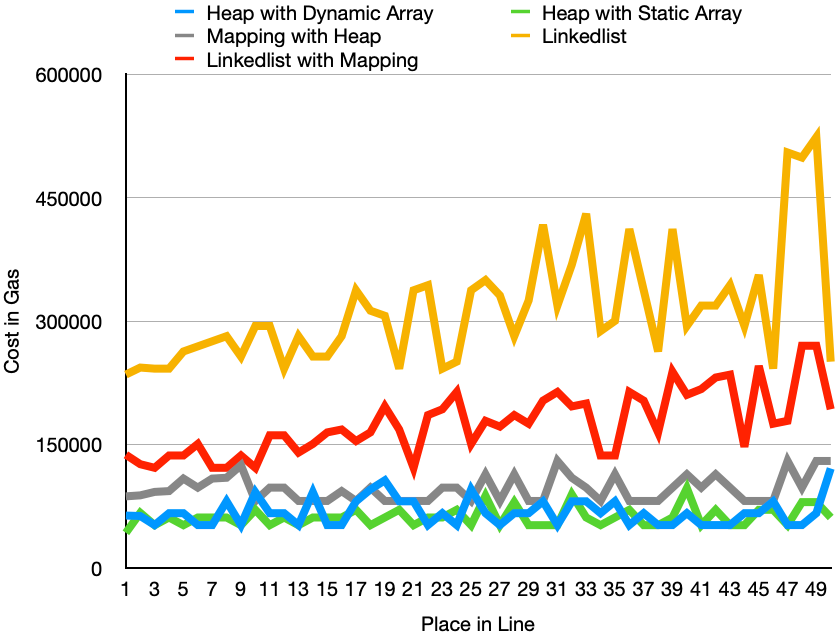
\includegraphics[width=1\textwidth]{fig/random_insertion.png}
\caption{\footnotesize{Gas costs for entering 50 items into five different priority queues.}  \label{fig:random_insertion}}
\end{figure}

% = = = = = = = = = = = = = = = = = = = = = = = = = = = = = = = = = = = = = = = =  %

Then, we called the \texttt{Dequeue()} function which iteratively removes the highest priority number from the priority queues (until the data structure is empty). The computational costs for dequeuing 50 unsigned integers in each priority queue are outlined in Table~\ref{tab:PQUnitTests}. These tests are performed using the current Ethereum gas metrics (block gas limit $=$11,741,495 and 1 gas $=$ 56 gwei)~\footnote{https://ethstats.net/}. The second column of the table shows the net gas consumption (the gasUsed value derived from transaction receipts) for removing 50 integers from each priority queues.  


% = = = = = = = = = = = =Gas costs and refunds for Dequeueing 50 integers from each PQ  = = = = = = = = = = = = =  %

\begin{table}[]
\centering
\begin{tabular}{|c|c|c|}
\hline

\textbf{\thead{Priority Queue}}    & \textbf{\thead{Net Cost in Gas\\ (\texttt{gasUsed})}}             & \textbf{\thead{Gas Refunds from Deleting a Storage\\(Manually Calculated)}} \\ \hline

% = = = = = = = = = = = = = = = = = = = = = = = = = = = = = = = = = = = = = = = = = = = = = = = = = = = = = = = = = = = = = = = = = = = = = = %
	\textbf{\thead{Heap with \\ Dynamic Array}}         				& 2,518,131            		      & 750,000                       \\ \hline
% = = = = = = = = = = = = = = = = = = = = = = = = = = = = = = = = = = = = = = = = = = = = = = = = = = = = = = = = = = = = = = = = = = = = = = %
	\textbf{\thead{Heap with \\ Static Array}}           				& 1,385,307                             & 750,000                      \\ \hline
% = = = = = = = = = = = = = = = = = = = = = = = = = = = = = = = = = = = = = = = = = = = = = = = = = = = = = = = = = = = = = = = = = = = = = = %
	\textbf{\thead{Mapping with \\ keys stored \\ in Heap}} 		& 2,781,684                            & 1,500,000                     \\ \hline
% = = = = = = = = = = = = = = = = = = = = = = = = = = = = = = = = = = = = = = = = = = = = = = = = = = = = = = = = = = = = = = = = = = = = = = %
	\textbf{Linked List}                       							& 557,085               	           & 1,200,000                      \\ \hline
% = = = = = = = = = = = = = = = = = = = = = = = = = = = = = = = = = = = = = = = = = = = = = = = = = = = = = = = = = = = = = = = = = = = = = = %
	\textbf{\thead{Linked List with \\ Mapping}}          				& 731,514              	     	  &  3,765,000                       \\ \hline
% = = = = = = = = = = = = = = = = = = = = = = = = = = = = = = = = = = = = = = = = = = = = = = = = = = = = = = = = = = = = = = = = = = = = = = %

\end{tabular}
\caption{\footnotesize{The gas metrics associated with dequeuing 50 items from five priority queues.}
\label{tab:PQUnitTests}}
\end{table}
% = = = = = = = = = = = = = = = = = = = = = = = = = = = = = = = = = = = = =  %

At the time of this writing, Ethereum transaction receipts only contain the net gas consumption (\texttt{gasUsed}) and we cannot obtain the value of the EVM's refund counter from inside the EVM~\cite{signer2018gas}. So in order to account for refunds inside each priority queue smart contract we calculate them manually; first we figure out exactly how much storage is being cleared when dequeuing the highest priority elements (\texttt{SSTORE} instruction) and then we multiply the number of storage slots cleared by 15,000 (see the last column of Table~\ref{tab:PQUnitTests}).

Note that in order to urge miners to process smart contracts with refunds, the accumulated gas refund can never exceed half the gas used up during computation~\cite{wood2014ethereum}. So at the end of a successful transaction, the amount of gas in the refund counter (capped at half the net gas used) is returned to the caller. Let's take a closer look at the last row of Table~\ref{tab:PQUnitTests}; gas that has been used for dequeuing 50 integers from the linked list with mapping priority queue is 731,514 and the gas limit has been set up to 11,741,495. Firstly, the caller will receive $(11,741,495 - 731,514) = 11,009,981$ units of unused gas. Also, the amount of refund we manually calculated based on the storage deletions is 3,765,000, and since this number is greater than half of he amount of gas that has been used in the contract ($3,765,000 > 731,514/2$), the refund generated will be $731,514/2 = 365,757$. So the caller of this transaction will eventually receive is $11,009,981 + 365,757 = 11,375,738$ units of gas.

%& \textbf{\thead{Net Cost\\in Gas\\ (\texttt{gasUsed})}}  
% = = = = = = = = = = = = = = = = = = = = = = = = = = = = = = = = = = = = =  %
% A little explanation on gas metrics (Mahsa: please let me know if this is still unclear:)


%First let's take a look at the following example:

%Suppose we have a smart contract which uses up 14,000 gas. The gas limit that we have set up is 20,000 gas. The smart contract also includes an SSTORAGE command.
%So, how much gas will the contract creator get back post computation?
%Firstly, they will get back (20,000-14,000) = 6,000 units of unused gas.
%Now, the SSTORAGE command has also been used, so theoretically they should get back 15,000 gas as well.
%However, the amount of gas that has been used in the contract is 14,000 and since 15,000 > 14,000/2, the REFUND generated will be 14,000/2= 7000.
%So the total gas that the creator is getting back in the end is 6000+7000 = 13,000.

% = = = = = = = = = = = = = = = = = = = = = = = = = = = = = = = = = = = = =  %


Based on our tests results, the \textit{linked list} and \textit{linked list with mapping} priority queues show the best performance in compared to the different heap implementations. In the next section, we explore the differences between the two different implementations of the linked list priority queue.


% = = = = = = = = = = = = = = = = = = = = = = = = = = = = = = = = = = = = =  %

\subsection{Linked List \textit{vs.} Linked List with Mapping}

There are two main ways to implement each of the \textit{linked list} and \textit{linked list with mapping} priority queues. In this section, we perform a comprehensive comparison between these two with the purpose choosing the proper data structure for implementing the call market.

%---------+++++++++++++++++++-----------------

\subsubsection*{Linked List.} Removing the highest priority element from the list can be done in two ways. We can use the \texttt{SELFDESTRUCT} operation to destroy the head node of the list (\ie smart contract) from the Ethereum blockchain and transfer its funds (if any) to a payable address (\eg the current block miner or the call market contract). Although the \texttt{SELFDESTRUCT} operation does not remove the initial byte code of the contract from the chain, but it frees up the state storage and refunds 24000 gas to the caller. Another design perspective is to only update the head pointer of the linked list and leave the previous head (\ie smart contract) on Ethereum blockchain when removing the highest priority element from the list. Although the first technique is a bit more costly (because it adds an extra operation \texttt{SELFDESTRUCT} to the \texttt{dequeue()} function), it results the in the less final net cost due to the 24000 gas refunds. Also, it is best to avoid storing unnecessary storage variables on chain. Table~\ref{tab:LLvsLLMapping} outlines different gas metrics for iteratively dequeuing the highest priority element from the two implementations of sorted linked lists that contain 50 unsigned integers.

%---------+++++++++++++++++++-----------------

\subsubsection*{Linked List with Mapping.} Similarly, linked list with mapping can be implemented in two ways. For dequeuing items from this priority queue we can use the \texttt{DELETE} method and remove the mapping element that contains the highest priority item from storage completely  \textbf{and} update the head and tail pointers of the list. Deleting a storage variable is identical to setting a non-zero variable to zero (\texttt{SSTORE} 0) that costs 20,000 gas but with15,000 refunded~\cite{wood2014ethereum}. So although the \texttt{DELETE} method refunds in 15000 gas, it is yet a gas-costly operation  as it increases the overall gas cost of the transaction. In another technique, we can only update the head and tail pointers of the linked list when dequeueing the highest priority items and not delete the mapping element associated with the previous pointers. As it can be seen in Table~\ref{tab:LLvsLLMapping}, this scheme consumes less gas to dequeue 50 unsigned integers from this priority queue with respect to the previous technique where we clear up the chain, however, leaving unnecessary storage data on chain is not a proper design practice.



% = = = = = = = = = = = = = = = = = = = = = = = = = = = = = = = = = = = = =  %
\begin{table}[]
\begin{tabular}{|c|c|c|c|c|}
\hline
\multirow{2}{*}{\textbf{Gas Metrics}}                        							& \multicolumn{2}{c|}{\textbf{Linked List}}           						& \multicolumn{2}{c|}{\textbf{Linked List with Mapping}}     					\\ \cline{2-5} 
% = = = = = = = = = = = = = = = = = = = = = = = = = = = = = = = = = = = = = = = = = = = = = = = = = = = = = = = = = = = = = = = = = = = = = =  = = = = = =  = = = = = = = = = = = = = = = =  = = = = = =  = = = = = = %
                                                                								& with \texttt{SELFDESTRUCT} 		& without \texttt{SELFDESTRUCT}                	& with \texttt{DELETE} 		& without \texttt{DELETE}              		\\ \hline                                                                                                                                                                                                                                                          % = = = = = = = = = = = = = = = = = = = = = = = = = = = = = = = = = = = = = = = = = = = = = = = = = = = = = = = = = = = = = = = = = = = = = =  = = = = = =  = = = = = = = = = = = = = = = =  = = = = = =  = = = = = = %
                  \textbf{\thead{Net Cost in Gas\\(\texttt{gasUsed})}}                        				& 557,085                    			& 721,370                     			& 731,514                     		& 334,689                      				\\ \hline
% = = = = = = = = = = = = = = = = = = = = = = = = = = = = = = = = = = = = = = = = = = = = = = = = = = = = = = = = = = = = = = = = = = = = = =  = = = = = =  = = = = = = = = = = = = = = = =  = = = = = =  = = = = = = %
 \textbf{\thead{Gas Refund \\from Deleting a Storage\\(Manually Calculated)}}            & 1,200,000                 				& 0                      					& 3,765,000                    		& 765,000                       				\\ \hline
% = = = = = = = = = = = = = = = = = = = = = = = = = = = = = = = = = = = = = = = = = = = = = = = = = = = = = = = = = = = = = = = = = = = = = =  = = = = = =  = = = = = = = = = = = = = = = =  = = = = = =  = = = = = = %

\end{tabular}
\caption{\footnotesize{}
\label{tab:LLvsLLMapping}}
\end{table}
% = = = = = = = = = = = = = = = = = = = = = = = = = = = = = = = = = = = = =  %


Based on Table~\ref{tab:LLvsLLMapping}, the linked list with \texttt{SELFDESTRUCT} appears to be a good candidate for the call market implementation. However, as it can be seen in Figure~\ref{fig:random_insertion}, the associated cost for inserting elements into this priority queue is significantly greater than the linked list with mapping as insertion is identical to creating new contracts. Accordingly, we choose to implement the call market with the linked list with mapping that uses the  the \texttt{DELETE} method to clear up the chain every time the highest priority element is removed from the list. In overall this priority queue introduces a moderate gas cost for both insertion (\ie order submission) and removal (\ie matching the orders). 



% = = = = = = = = = = = = = Experimentations = = = = = = = = = = = = = = = = = = =  %

\section{Experimentations}
 
As mentioned in~\ref{sec:callmarket}, Our system treats the time as discrete and not continuous; upcoming orders are accumulated over predetermined time intervals and are processed in batch instead of serially in order of receipt. The trading day is divided into frequent but discrete time intervals; every time the market opens traders submit their ask and bid order messages.  These orders are accumulated in a linked list with mapping priority queue and when the trading period is over, orders are matched against each other. The call market smart contract is written in 268 lines of Solidity, a high level programming language that is syntactically similar to Java~\cite{Ethereum41:online}, using the Truffle development framework and deployed on Ganache-CLI, Table~\ref{tab:callmarket_functions} represents the call market's primary operations.


% = = = = = = = = = = = = = = = = = = = = =Call market operations Table = = = = = = = = = = = =  = = = = = =  %
\begin{table}[]
\begin{tabular}{|l|l|}
\hline
\multicolumn{1}{|c|}{\textbf{Operation}} & \multicolumn{1}{c|}{\textbf{Description}}                            			\\ \hline

% = = = = = = = = = = = = = = = = = = = = = = = = = = = = = = = = = = = = = = = = = = = = = = = = = = = =  %
	DepositToken()                           & Deposits ERC20 standard compliant tokens in the call market contract \\ \hline
% = = = = = = = = = = = = = = = = = = = = = = = = = = = = = = = = = = = = = = = = = = = = = = = = = = = =  %
	DepositEther()                           	& Deposits Ethers in the call market contract                         			 \\ \hline
% = = = = = = = = = = = = = = = = = = = = = = = = = = = = = = = = = = = = = = = = = = = = = = = = = = = =  %
	OpenMarket()                             & Opens the market                                                    					 \\ \hline
% = = = = = = = = = = = = = = = = = = = = = = = = = = = = = = = = = = = = = = = = = = = = = = = = = = = =  %
	CloseMarket()                            & Closes the market                                                    					\\ \hline
% = = = = = = = = = = = = = = = = = = = = = = = = = = = = = = = = = = = = = = = = = = = = = = = = = = = =  %
	SubmitBid()                              & Inserts the upcoming bid order messages inside the priority queue    \\ \hline
% = = = = = = = = = = = = = = = = = = = = = = = = = = = = = = = = = = = = = = = = = = = = = = = = = = = =  %
	SubmitAsk()                              & Inserts the upcoming ask order messages inside the priority queue    \\ \hline
% = = = = = = = = = = = = = = = = = = = = = = = = = = = = = = = = = = = = = = = = = = = = = = = = = = = =  %
	MatchOrders()                           & Matches the orders against each other                                			\\ \hline
% = = = = = = = = = = = = = = = = = = = = = = = = = = = = = = = = = = = = = = = = = = = = = = = = = = = =  %
	ClaimTokens()                           & Transfers collateral tokens back to the trader                       			\\ \hline
% = = = = = = = = = = = = = = = = = = = = = = = = = = = = = = = = = = = = = = = = = = = = = = = = = = = =  %
	ClaimEther()                             & Transfers collateral Ethers back to the trader                       			\\ \hline
% = = = = = = = = = = = = = = = = = = = = = = = = = = = = = = = = = = = = = = = = = = = = = = = = = = = =  %
\end{tabular}
\caption{\footnotesize{Primary operations of the call market smart contract.}
\label{tab:callmarket_functions}}
\end{table}

% = = = = = = = = = = = = = = = = = = = = = = = = = = = = = = = = = = = = = = = = = = = = = = = = = = = =  %


To facilitate a safe exchange among buyers and sellers, we implement the Call Market smart contract in the form of a \textit{collateralized}; for market participants to be able to send bid and/or ask orders, they have to first supply tokens (depending on what ERC20 tokens they aim to trade) as collaterals by calling any of the  \texttt{DepositToken()} or \texttt{DepositEther()} methods. The collateralized call market acts as a payment guarantee so traders cannot default on payment or delivery of their assets. 

Followings outline results of the experiments we performed using Javascript and leveraging Mocha testing framework.
 
%============= Worst_Case_Matching_test.js Tables=================== %

 \subsection{Experiments}

%  = = = = = = = = = = % 


Table~\ref{tab:worst_case_matching} outlines the \texttt{Match()} function's computational costs and performance for three different implementations of the call market. We used three different designs of the linked list with mapping priority queue. (1) Every time a trade happens, we use the \texttt{DELETE} method to remove the mapping elements that contains best bid and ask orders from storage completely \textbf{and} update the head and tail pointers of the list. (2) We only update the pointers of the priority queue and do not remove the best bid and ask orders during the entire matching process. Instead we destroy the priority queue smart contract~\footnote{We execute a public function defined in the priority queue smart contract which itself calls the \texttt{self-destruct()} operation and transfers its funds (if any) to the call market contract.} once the matching is completed. (3) In the last implementation, we allow the matching process to be completed and do not clear any on chain data. As it can be seen in Table~\ref{tab:worst_case_matching}, the \texttt{Match()} operation shows a better performance when killing the priority contract and/or not clearing data from the chain. Although deleting the priority queue contract adds an extra external call to the \texttt{Match()} function and should technically increase the gas cost, the 24000 gas refunds from \texttt{SELFDESTRUCT} would compensate the cost. So it can still match as same number of orders (before running out of gas)as in the no on chain clearing implementation. The last column of Table~\ref{tab:worst_case_matching} reflects the gas cost for matching 1000 pairs of bids and asks for which we set the block gas limit to the maximum of  $2^{53}$ (the Javascript's max safe integer).

Note that this is a \textit{worst case matching} test where all bids and asks are submitted as marketable limit orders with specified prices that would be filled undoubtedly, performed using the current Ethereum gas metrics (block gas limit $=$11,741,495 and 1 gas $=$ 56 gwei)~\footnote{https://ethstats.net/}. 

% = = = = = = = = = = = =Worst Case Matching on Linkedlist With Mapping Table = = = = = = = = = = = = =  %

\begin{table}[]
\centering
\begin{tabular}{|c|c|c|c|}
\hline

\textbf{\thead{Linked List with Mapping}}    & \textbf{\thead{Maximum Number \\ of \\ Matched Orders}}      & \textbf{\thead{Net Cost\\in Gas}}          & \textbf{\thead{Net Cost in Gas\\ for \\ 1000 Pairs \\ of Orders}}    \\ \hline

% = = = = = = = = = = = = = = = = = = = = = = = = = = = = = = = = = = = = = = = = = = = = = = = = = = = = = = = = = = = = = = = = = = = = = = = = = = = = = = = = = = = = = = = = = = = =  = = = = = = = = = = = %
	\textbf{\thead{Clearing the Mapping Elements}}         			& 38 pairs                					& 5,372,679                   				& 457,326,935                      \\ \hline
% = = = = = = = = = = = = = = = = = = = = = = = = = = = = = = = = = = = = = = = = = = = = = = = = = = = = = = = = = = = = = = = = = = = = = = = = = = = = = = = = = = = = = = = = = = = =  = = = = = = = = = = = %
	\textbf{\thead{Destroying the Priority Queue Contract}}           	& 210 pairs	                     				& 5,304,211 							& 25,099,713				\\ \hline
% = = = = = = = = = = = = = = = = = = = = = = = = = = = = = = = = = = = = = = = = = = = = = = = = = = = = = = = = = = = = = = = = = = = = = = = = = = = = = = = = = = = = = = = = = = = =  = = = = = = = = = = = %
	\textbf{\thead{No On-chain Clearing}} 		                       	& 210 pairs							& 5,299,877							& 25,095,370				\\ \hline
% = = = = = = = = = = = = = = = = = = = = = = = = = = = = = = = = = = = = = = = = = = = = = = = = = = = = = = = = = = = = = = = = = = = = = = = = = = = = = = = = = = = = = = = = = = = =  = = = = = = = = = = = %

\end{tabular}
\caption{\footnotesize{}
\label{tab:worst_case_matching}}
\end{table}

% = = = = = = = = = = = = = = = = = = = = = = = = = = = = = = = = = = = = = = = = = = = = = = = = = = = =  %


%  = = = = = = = = = = % 
%Mahsa: Im not sure which of these tables are good for this section!?
%  = = = = = = = = = = % 



% = = = = = = = = = = = =Worst_Case_Matching Table = = = = = = = = = = = = =  %

\begin{table}[]
\centering
\begin{tabular}{|c|c|c|c|}
\hline

\textbf{\thead{Priority Queue}}    & \textbf{\thead{Maximum Number \\ of \\ Matched Orders}}      & \textbf{\thead{Net Cost\\in Gas}}          & \textbf{\thead{Net Cost in Gas\\ for \\ 1000 Pairs \\ of Orders}} \\ \hline

% = = = = = = = = = = = = = = = = = = = = = = = = = = = = = = = = = = = = = = = = = = = = = = = = = = = = = = = = = = = = = = = = = = = = = = %
	\textbf{\thead{Heap with \\ Dynamic Array}}         				& 38 pairs                & 5,372,679                   	& 457,326,935                      \\ \hline
% = = = = = = = = = = = = = = = = = = = = = = = = = = = = = = = = = = = = = = = = = = = = = = = = = = = = = = = = = = = = = = = = = = = = = = %
	\textbf{\thead{Heap with \\ Static Array}}           				& 42 pairs                & 5,247,636                  	& 333,656,805                       \\ \hline
% = = = = = = = = = = = = = = = = = = = = = = = = = = = = = = = = = = = = = = = = = = = = = = = = = = = = = = = = = = = = = = = = = = = = = = %
	\textbf{\thead{Mapping with \\ keys stored \\ in Heap}} 		& 46 pairs                & 5,285,275                     & 226,499,722                        \\ \hline
% = = = = = = = = = = = = = = = = = = = = = = = = = = = = = = = = = = = = = = = = = = = = = = = = = = = = = = = = = = = = = = = = = = = = = = %
	\textbf{Linkedlist}                       							& 152 pairs                & 5,495,265                     & 35,823,601                        \\ \hline
% = = = = = = = = = = = = = = = = = = = = = = = = = = = = = = = = = = = = = = = = = = = = = = = = = = = = = = = = = = = = = = = = = = = = = = %
	\textbf{\thead{Linkedlist with \\ Mapping}}          				& 86 pairs                 & 5,433,259                     & 62,774,170                        \\ \hline
% = = = = = = = = = = = = = = = = = = = = = = = = = = = = = = = = = = = = = = = = = = = = = = = = = = = = = = = = = = = = = = = = = = = = = = %

\end{tabular}
\caption{\footnotesize{}
\label{tab:worst_case_matching}}
\end{table}

% = = = = = = = = = = = =Clearing Mappings = = = = = = = = = = = = =  %

\section{Clearing Mappings}



To maintain the collateral balance of each market participant, we use two Solidity type one-to-one mapping that map Ethereum addresses to 256 bits unsigned integers; \texttt{TotalBalance} and \texttt{UnavailableBalance}. Once market closes and orders are matched, the \texttt{UnavailableBalance} needs to be cleared. However, since it is not possible to delete the entire mapping without knowing the keys~\footnote{https://solidity.readthedocs.io/en/v0.5.12/security-considerations.html}, clearing the \texttt{UnavailableBalance} mapping remains a challenging issue to solve . Here we provide a landscape of solutions for that.
%only individual keys and what they map to can be deleted.

\begin{enumerate}

%---------+++++++++++++++++++-----------------
\item \textbf{Creating a New Mapping Every Time the Market Opens.} Instead of clearing the \texttt{UnavailableBalance} of traders at the end of a matching process, we could create a new mapping every time the market opens. Note that using this solution, traders can only claim their funds (using the \texttt{ClaimEther()} and/or \texttt{ClaimToken} methods) only when the market is in state \texttt{Closed}. 


%---------+++++++++++++++++++-----------------
\item \textbf{Creating Custom Keys for the Mapping.} We can create custom keys for the mapping by defining a counter as a global variable inside the CallMarket smart contract. This counter is incremented at the end of the matching process. So instead of clearing the mapping, we only use another portion of it every time the market opens.


%---------+++++++++++++++++++-----------------
\item \textbf{Storing the Mapping in a Data-Contract.} Another design proposal is to create a smart contract every time the market opens, this data contract only stores the \texttt{UnavailableBalance} mapping and will be killed at the end of the matching process.



%---------+++++++++++++++++++-----------------
\item \textbf{Storing the Mapping keys in an additional Array.} Another common pattern is to create an additional array on top of the mapping and iterate over that. This array (\eg address[]) stores the traders' addresses and enables us to iterate over the mapping and delete individual keys and what they map to at the end of the matching process. Not that this is a gas-costly design pattern as we would need to maintain a secondary data structure.


%---------+++++++++++++++++++-----------------

\end{enumerate}

% = = = = = = = = = = = = = = = = = = = = = = = = = = = = = = = = = = = = = = = = = = = = = = = = = = = = = = = = = = = = = = = = = = = = =  %

% = = = = = = = = = = Design Details of PQs = = = = = = = = = = = = = = %
\section{Design Details of PQs}


%---------+++++++++++++++++++-----------------

\subsection{Mapping with Keys Stored in a Heap}\label{sec:mapping_heap}

To store the orders, here we use Solidity mapping that map orders' ids (256-bit integers) to order structs with their variables of different types. The mapping keys are then stored in a sorted heap that is implemented with a dynamic storage array. Every time a trade happens; (i) the mapping keys associated with the best bid and ask orders are deleted from the heap and the heap is re-sorted, and (ii) the mapping elements containing the best bid and ask orders are deleted from storage completely which refund 15000 gas~\cite{wood2014ethereum}. Deleting the mapping elements is yet a gas-costly operation which lowers down the maximum number of orders the \texttt{Match()} function could handle in this case.~\footnote{Every order structs contains multiple variables of different types and removing them from storage is identical to setting multiple variables to zero.} However, we clear the mapping element once a trade happens in our design as leaving unnecessary data is not a proper design practice.

%---------+++++++++++++++++++-----------------
\subsection {Linkedlist}
Every time a trade happens, we use the \texttt{SELFDESTRUCT} operation to remove the nodes (\ie smart contracts) containing the best bid and ask orders from the Ethereum blockchain. When a node is deleted, it transfers its funds (if any) to the payable address of the CallMarket contract that has been previously passed to it as a constructor argument. Also, removing a smart contract from the Ethereum blockchain refunds 24000 gas to the caller.


%---------+++++++++++++++++++-----------------
\subsection {Linkedlist with Mapping}
Every time a trade happens when the \texttt{Match()} function is executed, the best bid and ask orders need to be removed from the data structures. We could do this in two different ways; (i) update the head and tail pointers of the linkedlist and/or (ii) removing the mapping elements that contain the best bid and ask orders from storage completely as well as updating the pointers of the linkedlist. \par
For the same reason we mentioned in~\ref{sec:mapping_heap}, we clear the best bid and ask order structs from the mapping every time a trade happens as well as updating the pointers.



% = = = = = = = = = = = = = = = = = = = = = = = = = = = = = = = = = = = = = = = = = = = = = = = = = = = = = = = = = = = = = = = = = = = = =  %

% = = = = = = = = = = = =Closing and Reopening the Market = = = = = = = = = = = = =  %

\section{Closing and Reopening the Market}

% We use one-shot market for the sake of our performance tests on different data structures. and once we have all the numbers we can think about iterated market.

At the end of the trading period, the market needs to be closed and reopened. However, there is no automatic process to called an Ethereum function and contracts can only run when a function is called. 

%when to close the market?
%What time period?


% = = = = = = = = = = = =How to enforce time on on the Ethereum blockchain? = = = = = = = = = = = = =  %

\subsection{Enforcing Time on the Blockchain}

% We want the market to run on a periodic schedule => it is difficult for market participants to call the \texttt{Close()} function periodically.

% However there are incentives for them to do so: (i) they get paid and refunded (financial incentives), and (ii) Closing the market allow market participants to open it again and start their trading activities

% Another solution pattern to enforce the time is to use the Ethereum Alarm Clock 


% = = = = = = = = = = = =Who Pays the Cost for Closing and Reopening the Market?= = = = = = = = = = = = =  %

\subsection{Who Pays the Cost for Closing and Reopening the Market?}

We think it is useful to explore the landscape of possible designs for closing the market. 

\begin{enumerate}

%= = = = = = Miners Close the Market = = = = = = =%


\item \textbf {Miners Close and Reopen the Market.} The difference between the best bid and ask prices is called the \textit{bid-ask spread}. In our design, when the trade occurs between the the highest bid (the highest amount a buyer is willing to pay for an asset) and lowest ask (the lowest amount a seller is willing to accept for an asset) orders, the bid-ask spread is paid to the miner. There are possibilities that (i) no trade occurs or (ii) the bid-ask spread is zero (\ie the best bid and best ask prices are identical). So there is enough economic incentive for the the miner to execute the \texttt{CloseMarket()} function and get refunded as the refund amount could be potentially higher than the bid-ask spread. 



% = = = = = = = = = =Processing Orders in Groups= = = = = = = = = = = = = = = %

\item \textbf{Processing Orders in Groups.} Another solution pattern is to process certain number of bid and ask orders upon every execution of the \texttt{CloseMarket()} function rather than treating them as one substantial transaction. A market participant $P_i$ would process $n$ orders from the previous market (\texttt{CloseMarket(n)}) when sending new orders to the current market. This process continues until all the orders in the previous markets are processed. % incentive? => contribution to the community!?
 



%= = = = = =  = =  =  Meta txs =  = = = = = = = = =%

\item \textbf {Using the Meta Transactions.} Meta transactions enable users to execute Ethereum functions without paying the gas. Rather than spending gas, users sign their intended action using their private keys and broadcast it to the network with no cost. A third party process (\textit{a relayer}) then crafts the actual transaction on user's behalf, sends the transaction to the Ethereum blockchain, and charges the base contract with the associated fees (see Figure~\ref{fig:meta_tx}). The required gas to pay for the \texttt{Match()} function could be collected as fees. So market participants are charged with certain amounts of fees every time they submit an order, these fees are accumulated in the CallMarket contract and will be used to pay for executing the \texttt{CloseMarket()} function.

% = = = = = = = = = = = =meta_tx Figure = = = = = = = = = = = = =  %

\begin{figure}[htb!p]
\centering
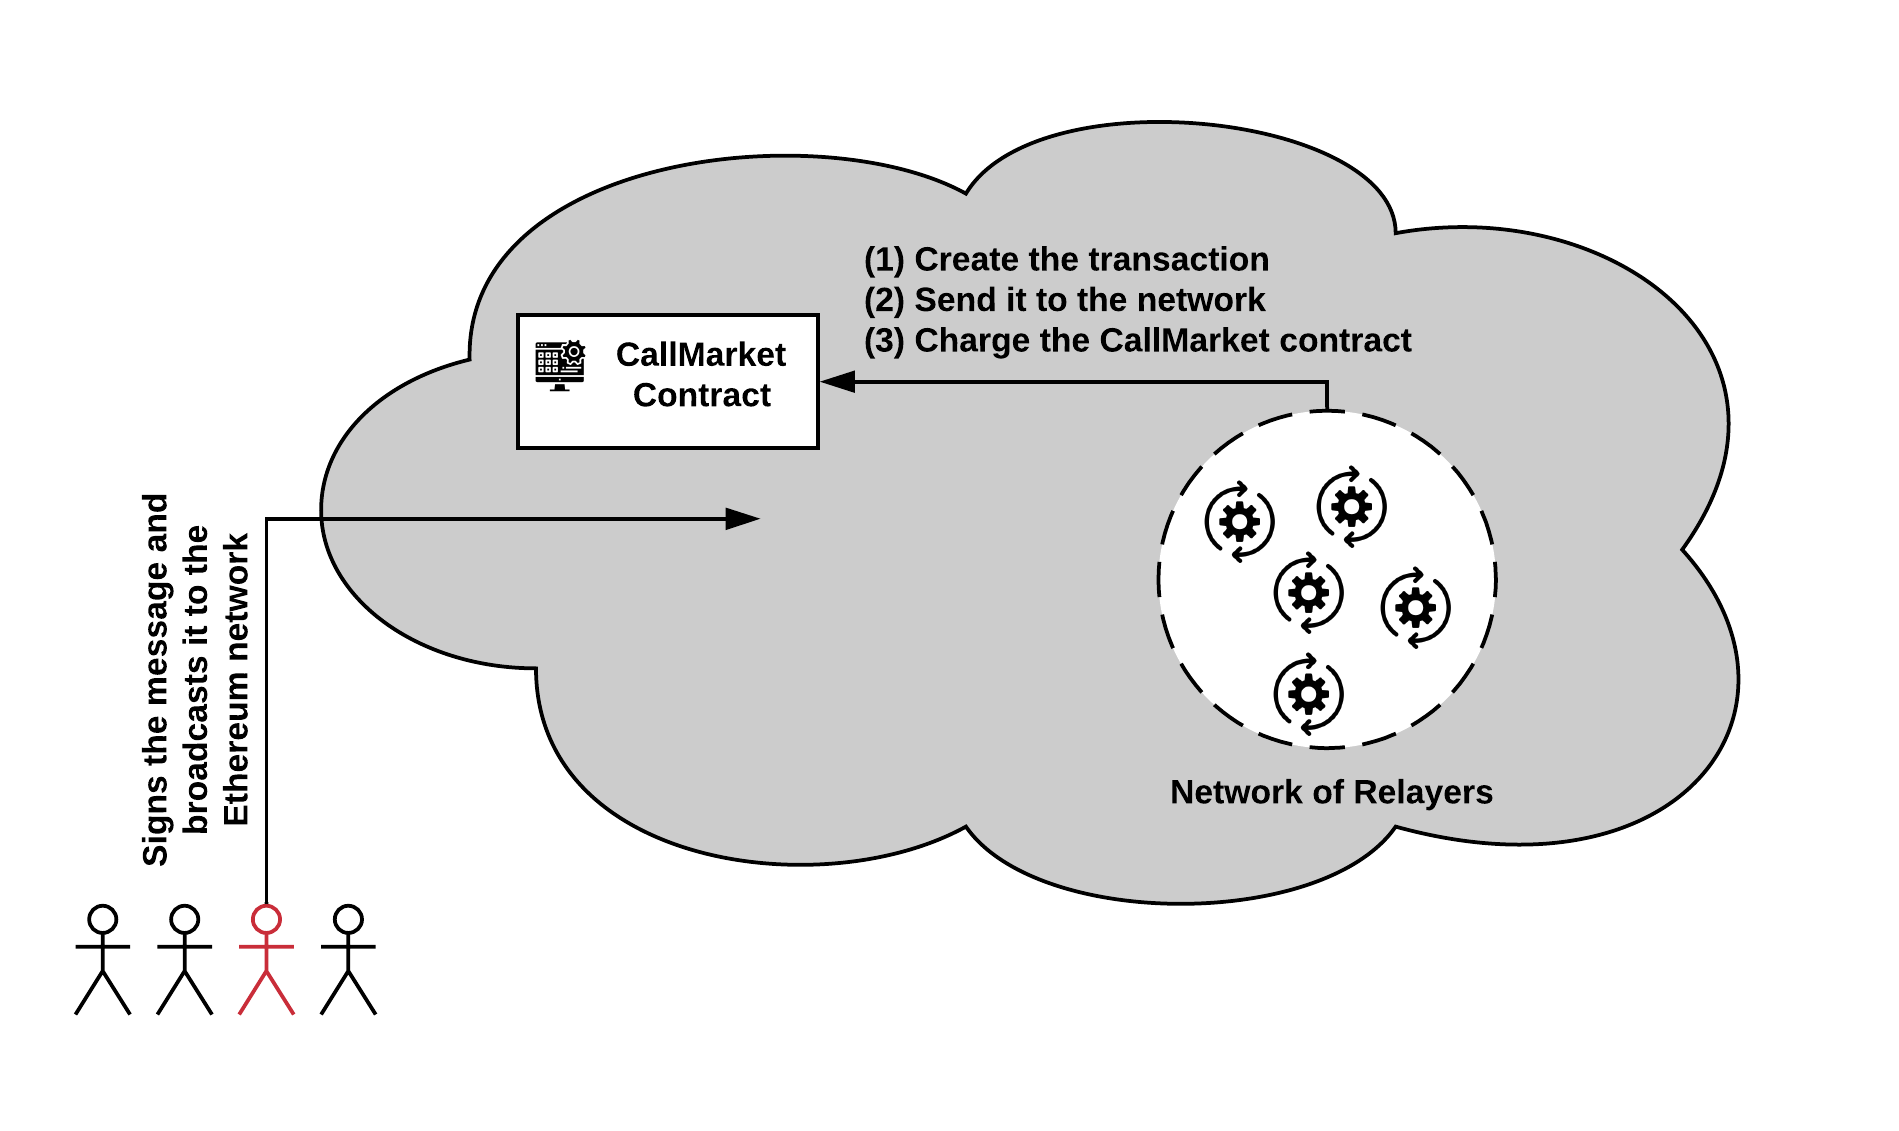
\includegraphics[width=0.8\textwidth]{fig/meta_tx.png}
\caption{\footnotesize{}  \label{fig:meta_tx}}
\end{figure}

% = = = = = = = = = = = = = = = = = = = = = = = = = = = = = = = = = %

%= = = = = =  = =  =  Users close and get refunded with the contract funds (collected as fees during order submissions) =  = = = = = = = = =%

\item \textbf{Using the "Contract Pays" Model.} An alternative solution is to design the market such that the last person to submit an order calls the \texttt{CloseMarket()} function, but in contrast to a normal transaction (where the person initiating the transaction must pay the fee), here the CallMarket contract pays the cost for closing the market and matching the orders respectively. To enforce this design we can use Solidity function modifiers; every time a new order is submitted, a function modifier checks whether (i) the auction period has to end and/or (ii) the maximum number of total orders has reached. If any of these two conditions are met, the \texttt{CloseMarket()} will be called. Again, market participants are charged with certain amounts of fees every time they submit an order, these fees are accumulated in the CallMarket. Once the \texttt{CloseMarket()} is successfully executed and orders are matched, the contract transfers its funds to that person. Note that here the person must still have enough gas to cover the execution of the transaction as the funds will be only transferred after the transaction is fully executed. However, market participants are incentivized to do so as they may receive more ethers than they have spent.

%= = = = = =  = =  =  Rollups=  = = = = = = = = =%

\item \textbf{Using Rollups.} Rollup is a scaling method that moves the storage and computation of the smart contracts off-chain while maintaining the transaction data on the main chain as call-data. In this technique, any Ethereum user can act as a validator; they can execute the \texttt{CloseMarket()}function and only post the new state of the contract (the updated balance of traders) in the form of \textit{assertions} to the main chain. Rollups improve scalability, provide faster and cheaper execution of the contracts, and eliminate the gas limit as the contract is no longer executed on-chain.
In the followings we briefly discuss different rollup proposals and techniques. Each approach uses a different method to ensure correction of assertions:


\begin{itemize}

\item \textbf{{Non-interactive Rollups.}} In this rollup technique, assertions are posted together with a validity proof that would be later used by validators to check if the \texttt{CloseMarket()} function has been executed correctly. ZK-Rollup scheme is one of the solutions that uses ZK-SNARKs to prove the validity of the assertions in zero-knowledge. ZK proofs are quick and cheap to verify but they are expensive and time consuming to generate. These proofs could be generated (i) for free or (ii) the CallMarket contract could collect proportional fees for every trade that is successfully executed.

\item \textbf{{Optimistic Rollups.}} In this scheme, assertions are assumed to be valid if there is no dispute posted about them with a certain window of time (a.k.a. "the challenge period'). Here, dispute resolution is a gas-costly method as the CallMarket contract would have to emulate the transaction on-chain to ensure the correctness the assertion. This scheme introduces a tradeoff between privacy and performance as all the assertions are publicly available and accessible. However, here the new state only reflects the updated balances of traders and no secret is involved. 

\item \textbf {{Multi-round Interactive Rollups.}} In this design paradigm, \textit{pending assertions} are posted on-chain and they are open to dispute. Once the challenge period is over and no challenge is submitted, the assertion is confirmed and the CallMarket contract transitions to the new state (\ie updates traders' balances). This scheme takes the overhead for the CallMarket contract to execute the \texttt{Close()} on-chain by using rounds to the dispute resolutions. The two parties (asserter and challenger) must run an interactive protocol and the CallMarket smart contract would have to act as a referee and decides which party's claim is true. Arbitrum is an example of multi-round interactive rollups that uses an efficient challenge-based protocol to penalize the dishonest parties~\cite{kalodner2018arbitrum}. 

\end{itemize}

%= = = = = =  = =  =  SGX=  = = = = = = = = =%

\item \textbf{{Using Trusted Execution Environments.}} Another way of achieving execution of the \texttt{CloseMarket()} function is incorporating the Ethereum blockchain into the Trusted Execution Environments (TEEs) and decoupling the contract execution from consensus mechanism. TEEs enable secure execution of applications in an isolated processing environment called the \textit{enclave}. Here, the enclave could execute the \texttt{CloseMarket()} function off-chain in TEEs and publish an on-chain attestation Quote to the CallMarket contract. The contract then verifies the correctness of the Quote and if validated correctly, it transitions to the new state. Ekiden is an example that uses Intel SGX to solve the scalability and confidentiality issues with the smart contract execution~\cite{cheng2019ekiden}. A drawback of this scheme is in order to achieve confidentiality-preserving smart contracts we have to trust a trusted party in the form of the hardware manufacturer (\eg Intel).


\end{enumerate}


% = = = = = = = = = = = = = = = = = = = = = = = = = = = = = = = = = = = = = = = = = = = = = = = = = = = = = = = = = = = = = = = = = = = = =  %










% = = = = = = = = = = = =Notes Discussed in Meetings = = = = = = = = = = = = =  %

% Our two competitors are Uinswap and Loopring (that uses ZK roll ups):
% 	1- Uniswap: we can argue that in traditional markets we have various traditional exchanges. Each of these exchanges have different trading rules and designs which work for different traders.
%	2- Loopring:
%		2-1: Barrier to entry: In order for a trader to trade specific ERC20 on Loopring, Loopring has to agree to support that token. It might not be difficult and they probably approve the token as long as it is standard compliant.
%		2-2: ZK proofs are quick and cheap to verify but they are expensive and time consuming to generate: (1) now they are generating these proofs for free but later they charge traders for doing that. (2) Looping does not probably generate these proofs per every block so the settlement and 				clearing is not happening per block. So we have faster clearing and settlement as we clear everything per block. 
% 		2-3: Loopring is non-custodial, meaning that the money moves only when the proofs come, so there is a latency in transferring funds to the traders.


% The heap with dynamic array can do 26 pairs of matches at worst case matching whereas Linkedliat does 90 pairs. So if we want to cap the orders over 4 PQs, we’re basically increasing the heap size which makes match more expensive for nothing (every time a match happens and the root is deleted the whole heap is reheapified)

% There will be no ties as we use 2 counters for buy and sell orders. These counters are concatenated them with the price. So we somehow enforce time priority


% = = = = = = = = = = = = = = = = = = = = = = = = = = = = = = = = = = = = = = = = = = = = = = = = = = = = = = = = = = = = = = = = = = = = =  %

% = = = = = = = = = = = = = = = = = = = = = = = = = = = = = = = = = = = = = = = = = = = = = = = = = = = = = = = = = = = = = = = = = = = = =  %
%The tables I changed after estimateGas, Not sure which ones to keep. Should talk to Jeremy 



% = = = = = = = = = = = =Gas costs and refunds for Dequeueing 50 integers from each PQ  = = = = = = = = = = = = =  %

\begin{table}[]
\centering
\begin{tabular}{|c|c|c|c|c|}
\hline

\textbf{\thead{Priority Queue}}    & \textbf{\thead{Net Cost\\in Gas}}      & \textbf{\thead{Total Cost\\in Gas\\(From \texttt{estimateGas})}}      & \textbf{The Difference}    & \textbf{\thead{Gas Refund \\(Manually Calculated)}} \\ \hline

% = = = = = = = = = = = = = = = = = = = = = = = = = = = = = = = = = = = = = = = = = = = = = = = = = = = = = = = = = = = = = = = = = = = = = = %
	\textbf{\thead{Heap with \\ Dynamic Array}}         				& 2,518,131               & 3,283,480		& 765,349             & 750,000                       \\ \hline
% = = = = = = = = = = = = = = = = = = = = = = = = = = = = = = = = = = = = = = = = = = = = = = = = = = = = = = = = = = = = = = = = = = = = = = %
	\textbf{\thead{Heap with \\ Static Array}}           				& 1,385,307                & 2,150,625     	& 765,318             & 750,000                      \\ \hline
% = = = = = = = = = = = = = = = = = = = = = = = = = = = = = = = = = = = = = = = = = = = = = = = = = = = = = = = = = = = = = = = = = = = = = = %
	\textbf{\thead{Mapping with \\ keys stored \\ in Heap}} 		& 2,781,684                & 4,316,229       	& 1,534,545           & 1,500,000                     \\ \hline
% = = = = = = = = = = = = = = = = = = = = = = = = = = = = = = = = = = = = = = = = = = = = = = = = = = = = = = = = = = = = = = = = = = = = = = %
	\textbf{Linked List}                       							& 557,085               	& 1,772,085      	& 1,215,000           & 1,200,000                      \\ \hline
% = = = = = = = = = = = = = = = = = = = = = = = = = = = = = = = = = = = = = = = = = = = = = = = = = = = = = = = = = = = = = = = = = = = = = = %
	\textbf{\thead{Linked List with \\ Mapping}}          				& 731,514              	& 3,731,514       	& 3,000,000     	  &  3,765,000                       \\ \hline
% = = = = = = = = = = = = = = = = = = = = = = = = = = = = = = = = = = = = = = = = = = = = = = = = = = = = = = = = = = = = = = = = = = = = = = %

\end{tabular}
\caption{\footnotesize{The gas metrics associated with dequeuing 50 items from five priority queues.}
\label{tab:PQUnitTests}}
\end{table}
% = = = = = = = = = = = = = = = = = = = = = = = = = = = = = = = = = = = = =  %

% = = = = = = = = = = = = = = = = = = = = = = = = = = = = = = = = = = = = =  %
\begin{table}[]
\begin{tabular}{|c|c|c|c|c|}
\hline
\multirow{2}{*}{Gas Metrics}                        							& \multicolumn{2}{c|}{Linked List}           						& \multicolumn{2}{c|}{Linked List with Mapping}     					\\ \cline{2-5} 
% = = = = = = = = = = = = = = = = = = = = = = = = = = = = = = = = = = = = = = = = = = = = = = = = = = = = = = = = = = = = = = = = = = = = = =  = = = = = =  = = = = = = = = = = = = = = = =  = = = = = =  = = = = = = %
                                                                						& with \texttt{SELFDESTRUCT} 		& without \texttt{SELFDESTRUCT}                	& with \texttt{delete} 		& without \texttt{delete}              		\\ \hline                                                                                                                                                                                                                                                          % = = = = = = = = = = = = = = = = = = = = = = = = = = = = = = = = = = = = = = = = = = = = = = = = = = = = = = = = = = = = = = = = = = = = = =  = = = = = =  = = = = = = = = = = = = = = = =  = = = = = =  = = = = = = %
                   Net Cost in Gas                          					& 557,085                    			& 721,370                     				& 731,514                     	& 334,689                      				\\ \hline
% = = = = = = = = = = = = = = = = = = = = = = = = = = = = = = = = = = = = = = = = = = = = = = = = = = = = = = = = = = = = = = = = = = = = = =  = = = = = =  = = = = = = = = = = = = = = = =  = = = = = =  = = = = = = %
\thead{Total Cost in Gas \\ (from \texttt{estimateGas})} 		& 1,772,085                  			& 736,370                  					& 3,731,514                     	& 1,099,689                       				\\ \hline
% = = = = = = = = = = = = = = = = = = = = = = = = = = = = = = = = = = = = = = = = = = = = = = = = = = = = = = = = = = = = = = = = = = = = = =  = = = = = =  = = = = = = = = = = = = = = = =  = = = = = =  = = = = = = %
		    The Difference                                             		& 1,215,000                  			& 15,000                      				& 3,000,000                    	& 765,000                       				\\ \hline
% = = = = = = = = = = = = = = = = = = = = = = = = = = = = = = = = = = = = = = = = = = = = = = = = = = = = = = = = = = = = = = = = = = = = = =  = = = = = =  = = = = = = = = = = = = = = = =  = = = = = =  = = = = = = %

\end{tabular}
\caption{\footnotesize{}
\label{tab:LLvsLLMapping}}
\end{table}
% = = = = = = = = = = = = = = = = = = = = = = = = = = = = = = = = = = = = =  %




%======================================== %

% = = = = = = = = = = = = = = = = = = = = = = = = = = = = = = = = = = = = = = = = = =

\section{Concluding Remarks}


 
%\subsubsection*{Acknowledgements.} J. Clark thanks ...

































